\documentclass[aspectratio=169]{beamer}

\usepackage[english]{babel}
\usepackage[utf8]{inputenc}
\usepackage[T1]{fontenc}
\usepackage{lmodern}

\newcommand{\Author}{Sebastian Einsiedler}
\newcommand{\Title}{Programming for Biologist}
\newcommand{\SubTitle}{Fundamental building blocks}

\title{\Title}
\subtitle{\SubTitle}
\author{\Author}

\usepackage{amsmath, amssymb}
\usepackage{enumerate}
\usepackage[table]{xcolor}
\usepackage[singlespacing]{setspace}
\usepackage{hyperref}
\hypersetup{
	bookmarks=true,
	unicode=true,
	pdfauthor = {\Author},
	pdftitle = {\Title},
	pdfsubject = {\Title},
	pdfsubject = {\Author, \Title, \SubTitle Python, Programming, Programming for biologists, presentation},
	colorlinks = true,
	linkcolor = {blue!50!black},
	filecolor = {red!50!black},
	urlcolor = {blue!75!black}
}
\usepackage{csquotes}

\usepackage{footnotebackref}
\usepackage{longtable}
\usepackage{booktabs}
\usepackage{graphicx}
\usepackage{tikz}
\usepackage{listings}

\setbeamertemplate{navigation symbols}{}
\setbeamertemplate{footline}{
	\hspace{2ex}
	\insertshorttitle
	: \hspace{3em}
	\insertsectionhead
	\hfill
	\insertframenumber /
	\inserttotalframenumber
	\hspace{2ex}
	\vspace{2ex}
}

\setcounter{tocdepth}{1}
\hypersetup{bookmarksdepth = 3}

\begin{document}

\usebackgroundtemplate{
\includegraphics[width=\paperwidth]{img/Title.png}}
\begingroup
\setbeamertemplate{footline}{}
\begin{frame}{\phantom{Title}}

	\vskip 6em
	\color{white}
	\LARGE \Title{}
	\newline
	\large
	\SubTitle{}
	
	\vskip 5em
	\small
	\Author{}
	and 
	\color{white}{Eduard Maier} \\
	RG Neurobiology of maternal care \\
	Department Neuropeptide research in psychiatry
}
\end{frame}
\endgroup

\usebackgroundtemplate{
\includegraphics[width=\paperwidth]{img/Body.png}}

\section{Table of contents}
\begin{frame}
	\frametitle{Table of contents}
	\tableofcontents
\end{frame}

\section{Recall}
\begin{frame}{Recall}{Concepts}
\begin{itemize}
	\item Memory cells
	\item Types
	\item Operators
	\item Variables
\end{itemize}
\end{frame}

\begin{frame}{Recall}{Algorithm}
\setbeamertemplate{itemize/enumerate body begin}{\tiny}
\setbeamertemplate{itemize/enumerate subbody begin}{\tiny}
\setbeamertemplate{itemize/enumerate subsubbody begin}{\tiny}

Yesterdays algorithm:

\begin{enumerate}
\item {Open the units-file}
\item {Figure out how many units there are}
\item {Figure out when the last spike occurs in seconds}
\item {Create a column with one entry for every second between 0 and the last spike occurrence.}
\item {Use this column to begin a table}
\item {For every unit:}
\begin{enumerate}
	\item {Create a column containing the same amount of entries as the second-column}
	\item {Fill the list with 0s}
	\item {For every row in the unit file:}
	\begin{enumerate}
		\item {Find the second to which the spike belongs}
		\item {Increase the entry in the column corresponding to this second}
	\end{enumerate}
	\item {Add the column to the table}
\end{enumerate}
\item {Open the immobility file}
\item {Create a column containing the same amount of entries as the second-column}
\item {For every second in the immobility-list:}
\begin{enumerate}
	\item {Mark as "Yes" if it is within an immobility phase otherwise mark as "No"}
\end{enumerate}
\item {Add the column to the table}
\end{enumerate}
\end{frame}

\section{Operators}
\begin{frame}{Operators}
\begin{tabular}{cllll}
\toprule
	Operator & Action & Example & Resulting value \\
\midrule
	= & Assign & a = 5 & 5\\
	+ & Addition & 3 + 4 & 7 \\
	- & Subtraction & 8 - 3 & 5 \\
	* & Multiplication & 2 * 3 & 6 \\
	** & Power of & 2 ** 3 & 8 \\
	/ & Division & 8 / 4 & 2 \\
\bottomrule
\end{tabular}

\pause
\vspace{2em}

Please solve the corresponding exercises in the materials.
\end{frame}

\section{Types}
\begin{frame}{Types}{Integers}

Recall integers:

\centering
\begin{tabular}{lllllllll}
	\toprule
	Bit        & 0   & 0  & 0  & 1  & 0 & 0 & 1 & 1 \\
	Represents & 128 & 64 & 32 & 16 & 8 & 4 & 2 & 1 \\ 
	Value      & 0   & 0  & 0  & 16 & 0 & 0 & 2 & 1 \\
	\midrule
\end{tabular}
\end{frame}

\begin{frame}{Types}{Float}

New floating point numbers:

\begin{figure}
	\centering
	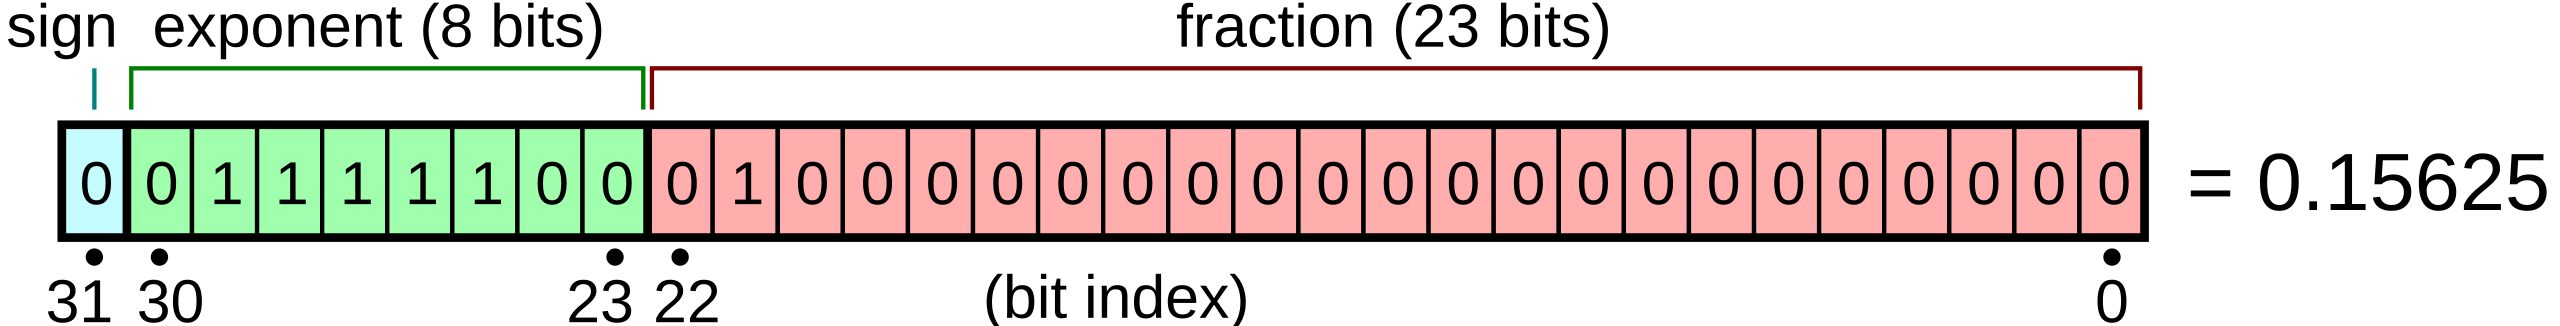
\includegraphics[width=0.8\textwidth]{img/Float.png}
	\caption{Example of a float: \url{https://commons.wikimedia.org/wiki/File:Float_example.svg}}
\end{figure}
\end{frame}

\begin{frame}{Types}{In binary}
\begin{tabular}{
	ll
	ll
	ll
	ll
	ll
	ll
}
	\toprule
	Type & Value
	&\multicolumn{2}{c}{Byte 4}
	&\multicolumn{2}{c}{Byte 3}
	&\multicolumn{2}{c}{Byte 2}
	&\multicolumn{2}{c}{Byte 1}\\
	\midrule
	8-bit integer & 42
	&&
	&&
	&&
	& 0010 & 1010 \\
	32-bit integer & 42
	& 0000 & 0000
	& 0000 & 0000
	& 0000 & 0000
	& 0010 & 1010 \\
	32-bit float & 42 
	& 0100 & 0010
	& 0010 & 1000
	& 0000 & 0000
	& 0000 & 0000 \\
	\bottomrule
\end{tabular}

\pause
\vspace{2em}
Let us now take a closer look at the float again:
\vspace{1em}

\begin{tabular}{
	l
	lll
	ll
	ll
	ll
}
	\toprule
	Binary
	& 0 
	& 1000 & 00100
	& 010 & 1000
	& 0000 & 0000
	& 0000 & 0000 \\
	\pause
	Content
	& sign  
	&\multicolumn{2}{l}{Exponent}
	&\multicolumn{6}{l}{Mantisse} \\
	\pause
	Int Value 
	& 0
	&\multicolumn{2}{l}{132}
	&\multicolumn{6}{l}{2621440}\\
	\pause
	Meaning
	& +
	& \multicolumn{2}{l}{\begin{math} 2^{5}\end{math}}
	& \multicolumn{6}{l}{\begin{math} 1.3125 \end{math}} \\
	\bottomrule
\end{tabular}
\end{frame}

\section{Types}
\begin{frame}[fragile]{Types}{In Python}

Switching types in Python:

\begin{lstlisting}[language=Python, frame=single]
number = 42
number_as_float = float(number)
number_as_int = int(number)
print(number_as_float)
print(number_as_int)
\end{lstlisting}

\pause
\vspace{2em}
\begin{itemize}
	\item Python does not have overflow errors
	\item Numpy has overflow errors
	\item All floats introduce rounding errors
\end{itemize}

\end{frame}

\begin{frame}{Booleans}{Bool creating operators}
\begin{tabular}{cllc}
\toprule
	Operator & Action & Example & Resulting value \\
\midrule
	== & checks if equal                     & 4 == 3      & False \\
	!= & checks if not equal                 & 4 != 3      & True  \\
	<  & checks if left is smaller           & 3 < 4       & True  \\
	<= & checks if left is smaller or equal  & 3 <= 4      & True  \\
	>  & checks if left is bigger            & 3 > 4       & False \\
	>= & checks if left is bigger or equal   & 3 >= 4      & False \\
	in & checks if left value is in right    & 1 in [1, 2] & True \\
	is & checks if both values are identical & 3 is 4      & False\\
\bottomrule
\end{tabular}

\vspace{2em}

Pleas use this operators to solve the exercises in the jupyter notebook.

\end{frame}

\begin{frame}{Booleans}{Bool using operators}
\begin{tabular}{cllc}
\toprule
	Operator & Action & Example & Resulting value \\
\midrule
	not & inverts a bool                     & not True       & False \\
	and & True if both values are True       & True and False & False\\
	or  & True if at least one value is True & True or False  & True  \\
\bottomrule
\end{tabular}

\vspace{2em}

Pleas use this operators to solve the exercise in the jupyter notebook.

\end{frame}

\begin{frame}{Mutable types}
\begin{itemize}
	\item Mutable types can be changed in place
	\item Mutable types are stored by reference
	\item Let us explore mutable on the example of list
\end{itemize}
\end{frame}

\begin{frame}[fragile]{Mutable types}{List}
\begin{lstlisting}[language=Python, frame=single]
# Creating a filled list
spike_numbers_unit_1 = [10, 12, 11, 9 ,10]
# Appending to a list
spike_numbers_unit_1.append(42)
# Remove an element from a list and get it back
last_spike_number = spike_numbers_unit_1.pop()
# Accessing a value in the list
spike_numbers_unit_1_second_3 = spike_numbers_unit_1[2]
\end{lstlisting}
\end{frame}

\begin{frame}[fragile]{Mutable types}{Example}
\begin{lstlisting}[language=Python, frame=single]
a = 4
a + 3
print(a)
\end{lstlisting}

Result: \pause \textquote{4}

\pause

\begin{lstlisting}[language=Python, frame=single]
a = [0.0, 4.5, 8.3]
a.pop()
a.append(42.0)
print(a)
\end{lstlisting}

Result: \pause \textquote{[0.0, 4.5, 8.3]}

\pause
\textquote{a} was changed by append and pop.

\end{frame}

\begin{frame}[fragile]{Mutable types}{Reference}

What does this mean:
\begin{lstlisting}[language=Python, frame=single]
spike_counter = 0
spike_counter_copy = spike_counter
\end{lstlisting}

\pause

What does this print?

\begin{lstlisting}[language=Python, frame=single]
spike_number_unit_1 = [12, 23, 35]
spike_number_unit_1_reference = spike_number_unit_1
spike_number_unit_1_reference[1] = 42
print(spike_number_unit_1)
\end{lstlisting}

Please predict what this code will print before executing it.

\end{frame}

\begin{frame}[fragile]{Mutable types}{Copy}

\begin{lstlisting}[language=Python, frame=single]
spike_number_unit_1 = [12, 23, 35]
spike_number_unit_1_reference = spike_number_unit_1.copy()
spike_number_unit_1_reference[1] = 42
print(spike_number_unit_1)
\end{lstlisting}

Please predict what this code will print before executing it.

\end{frame}

\section{Update our plan}
\begin{frame}{Update our plan}
\setbeamertemplate{itemize/enumerate body begin}{\tiny}
\setbeamertemplate{itemize/enumerate subbody begin}{\tiny}
\setbeamertemplate{itemize/enumerate subsubbody begin}{\tiny}

Updating our algorithm:

\begin{enumerate}
\item {Open the units-file}
\item {\begin{math} \checkmark \end{math}
	Figure out how many units there are:
	\textquote{number\_of\_units += 1}
}
\item {Figure out when the last spike occurs in seconds}
\item {\begin{math} \checkmark \end{math}
	Create a column with one entry for every second between 0 and the last spike occurrence:
	\textquote{second\_column = []} and \textquote{.append(second)}
}
\item {\begin{math} \checkmark \end{math}
	Use this column to begin a table:
	\textquote{table = [second\_column]}
}
\item {For every unit:}
\begin{enumerate}
	\item {\begin{math} \checkmark \end{math}
		Create a column containing the same amount of entries as the second-column:
		\textquote{unit\_column = second\_column.copy()}
	}
	\item {\begin{math} \checkmark \end{math}
		Fill the list with 0s:
		\textquote{unit\_column.append(0)}
	}
	\item {For every row in the unit file:}
	\begin{enumerate}
		\item {\begin{math} \checkmark \end{math}
			Find the second to which the spike belongs:
			\textquote{spike\_time >= second and spike\_time <= second + 1}
		}
		\item {\begin{math} \checkmark \end{math}
			Increase the entry in the column corresponding to this second
			\textquote{unit\_column[second] += 1}
		}
	\end{enumerate}
	\item {\begin{math} \checkmark \end{math}
		Add the column to the table:
		\textquote{table.append(unit\_column)}
	}
\end{enumerate}
\item {Open the immobility file}
\item {\begin{math} \checkmark \end{math}
	Create a column containing the same amount of entries as the second-column:
	\textquote{immobility\_column = second\_column.copy()}
}
\item {For every second in the immobility-list:}
\begin{enumerate}
	\item {\begin{math} \checkmark \end{math}
		Mark as "Yes" if it is within an immobility phase otherwise mark as "No":
		\textquote{immobility\_column[second] = second > immbolity\_phase\_begin and second < immoblitly\_phase\_end}
	}
\end{enumerate}
\item {\begin{math} \checkmark \end{math}
	Add the column to the table:
	\textquote{table.append(immobility\_column)}
}
\end{enumerate}
\end{frame}

\section{Strings}
\begin{frame}{Strings}
\begin{itemize}
	\item Text is organized in "character Strings"
	\item Python uses the type \textquote{str}
	\item \textquote{str} are not mutable
\end{itemize}

Pleas write a little bit of code to print your name.

\end{frame}

\section{Files}
\begin{frame}[fragile]{Files}

Please try out the following lines in your material and interpret the results:

\begin{lstlisting}[language=Python, frame=single, basicstyle=\footnotesize]
csv_file = open("./data_neuron/session_2023111501010_immobility.csv")
print(csv_file)
\end{lstlisting}

\pause
\vspace{0.5em}
Please try out the following lines in your material and interpret the results:

\begin{lstlisting}[language=Python, frame=single, basicstyle=\footnotesize]
csv_file = open("./data_neuron/session_2023111501010_immobility.csv")
content = csv_file.read()
print(content)
\end{lsisstlisting}

\pause
\vspace{0.5em}
Please try out the following lines in your material to write into a file:
\begin{lstlisting}[language=Python, frame=single, basicstyle=\footnotesize]
file_to_write = open("./write.txt", "w")
text_to_write = "Hello file!"
file_to_write.write(text_to_write)
\end{lstlisting}

\end{frame}

\section{Working with strings}
\begin{frame}[fragile]{Working with strings}

Please execute the following lines in your materials:

\begin{lstlisting}[language=Python, frame=single, basicstyle=\footnotesize]
csv_file = open("./data_neuron/session_2023111501010_immobility.csv")
content = csv_file.read()
lines = content.splie("\n")
print(lines)
\end{lstlisting}

\pause
\vspace{2em}
Please use what you have learned to split the first two lines into lists of elements.

\end{frame}

\section{Type conversions}
\begin{frame}[fragile]{Type conversions}

To convert types we use the type-name and the variable we wish to convert.

\begin{lstlisting}[language=Python, frame=single, basicstyle=\footnotesize]
String = "42"
Integer = int(String)
\end{lstlisting}

\vspace{2em}

Please use this knowledge to convert the values given in your materials.

\end{frame}

\section{Pseudo Code}
\begin{frame}{Pseudo Code}

\begin{itemize}
	\item Looks like "real" code
	\item Covers detailed ideas
	\item Usually used to write down ideas, before bothering with details
\end{itemize}

\pause

\vspace{2em}

Let us go over the example in the materials.

\end{frame}

\section{Other relevant types}
\begin{frame}[fragile]{Other relevant types}{Tuple}

Tuple are essentially non mutable lists.

\begin{lstlisting}[language=Python, frame=single]
tuple_1 = ("A", 42)
tuple_2 = "Foo", "bar", 48
print(tuple_1)
print(tuple_2)
\end{lstlisting}

\end{frame}

\begin{frame}[fragile]{Other relevant types}{Dict}

Dicts permit us to access values by keys.

\begin{lstlisting}[language=Python, frame=single, basicstyle=\footnotesize]
name_to_age = {
    "John Doe":  28,
    "Maria Musterfrau": 31,
    "Max Mustermann": 34,
    "Karl Dosenkohl": 19
}

name_to_age["Jane Doe"] = 27
age_john_doe = name_to_age["John Doe"]

# No let us get all the keys from the dict
keys = id_to_confusion.keys()
# This can be useful if we want to find a specific value
values = id_to_confusion.values()
\end{lstlisting}

\end{frame}

\begin{frame}[fragile]{Other relevant types}{Sets}

Mathematical sets are containers that contain a value only once.

\begin{lstlisting}[language=Python, frame=single]
tuple_for_set = {1, 2, 3, 3, 4}
new_set = set(tuple_for_set)
print(new_set)
\end{lstlisting}

\end{frame}

\section{Summary}
\begin{frame}{Summary}

This module we learned about:
\begin{itemize}
	\item Operators
	\item Type
\end{itemize}

\vspace{2em}

The current state of our algorithm can be found in the materials.

\end{frame}

\section{Question and answers}
\begin{frame}{Questions and answers}
\huge
\centering
Please ask any remaining questions now.
\end{frame}

\end{document}
